\chapter{Hệ thống EasyMesh của Mediatek}
\label{chapter:chapter-3}
\section{Tổng quan phần mềm EasyMesh}

\begin{figure}
\centering
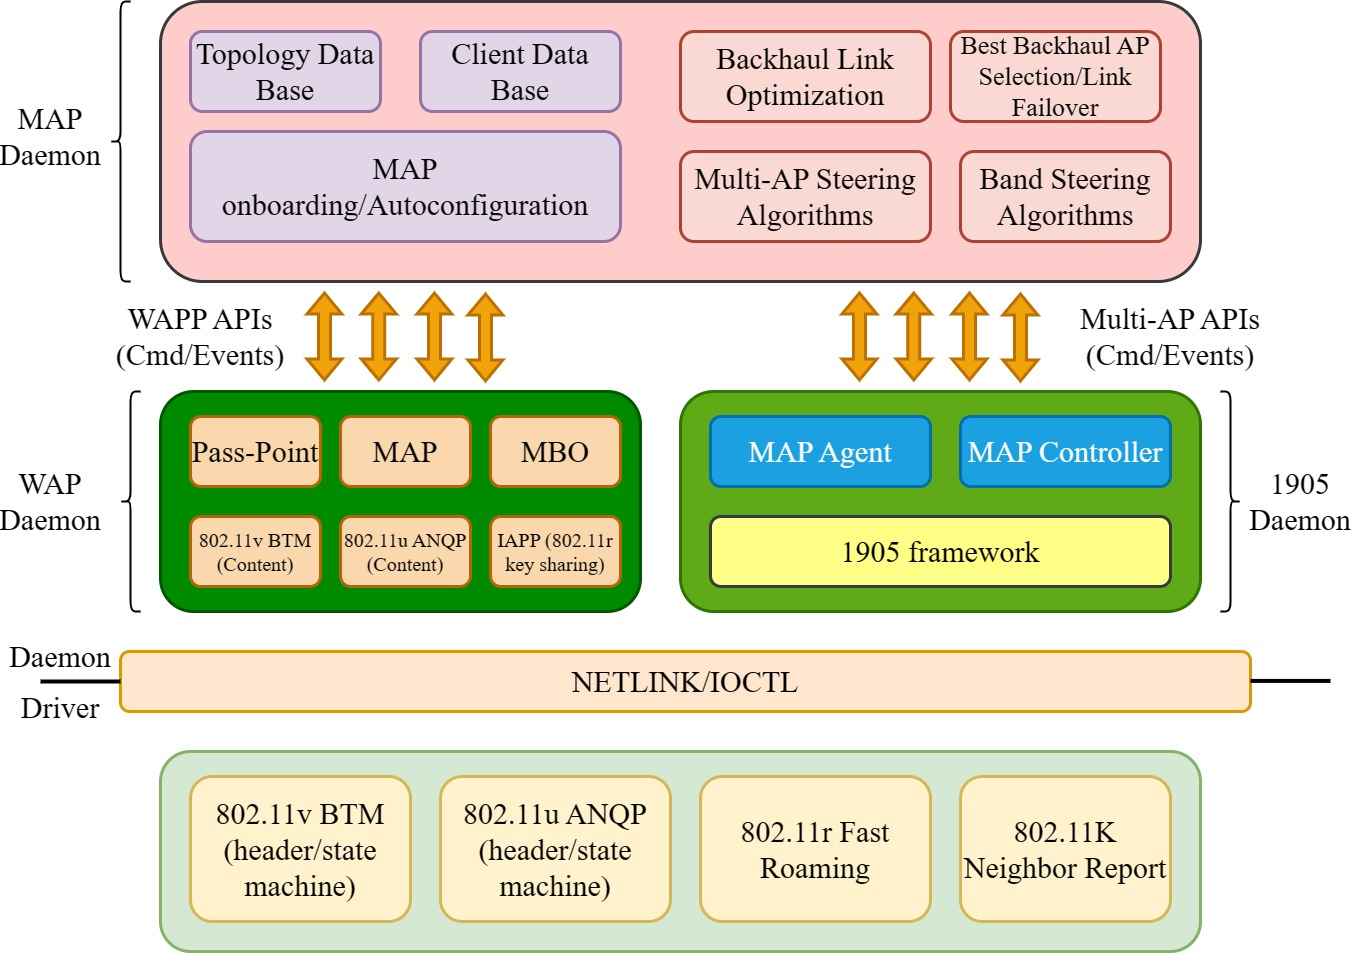
\includegraphics[width=0.8\textwidth]{mainmatter/images/MTK_ACH.jpg}
\caption{\label{fig:EasyMeshHi}Thiết kế phần mềm của EasyMesh}
\end{figure}

\section{Thuật toán chọn kênh}

Thuật toán chọn kênh thường bao gồm các bước sau:

\begin{itemize}
    \item \textbf{Quét phổ (spectrum scan / passive scan):}
    \begin{itemize}
        \item Driver quét các kênh trong băng tần (2.4GHz và 5GHz) để thu thập thông tin nhiễu, RSSI, CCA (Clear Channel Assessment), beacon từ các AP khác.
    \end{itemize}

    \item \textbf{Đánh giá độ nhiễu (interference):}
    \begin{itemize}
        \item Đo các chỉ số như:
        \begin{itemize}
            \item Tổng thời gian kênh bị chiếm dụng (channel busy time)
            \item Mức RSSI nền
            \item Số lượng BSSID phát hiện được
        \end{itemize}
    \end{itemize}

    \item \textbf{Ưu tiên kênh sạch (clean channel preference):}
    \begin{itemize}
        \item Kênh ít bị chiếm dụng, RSSI thấp, ít AP xung quanh sẽ được ưu tiên.
    \end{itemize}

    \item \textbf{Áp dụng các chính sách ưu tiên:}
    \begin{itemize}
        \item Kênh DFS (Dynamic Frequency Selection) có thể bị tránh nếu chưa được xác thực.
        \item Một số thiết bị tránh kênh chẵn/lẻ tùy thị trường (Regulatory Domain).
    \end{itemize}
\end{itemize}

\usetikzlibrary{shapes.geometric, arrows.meta, positioning}
\tikzstyle{startstop} = [rectangle, rounded corners, minimum width=3cm, minimum height=1cm,text centered, draw=black, fill=blue!20]
\tikzstyle{process} = [rectangle, minimum width=3cm, minimum height=1cm, text centered, draw=black, fill=green!20]
\tikzstyle{decision} = [diamond, minimum width=3cm, minimum height=1cm, text centered, draw=black, fill=orange!30]
\tikzstyle{arrow} = [thick, ->, >=stealth]

\section*{Lưu đồ thuật toán chọn kênh WiFi}

\begin{center}

\begin{tikzpicture}[node distance=2cm]

\node (start) [startstop] {Bắt đầu};
\node (scan) [process, below of=start] {Quét phổ (2.4/5GHz)};
\node (evaluate) [process, below of=scan] {Đánh giá độ nhiễu (RSSI, busy time, BSSID)};
\node (prefer) [process, below of=evaluate] {Ưu tiên kênh sạch};
\node (policy) [process, below of=prefer] {Áp dụng chính sách (tránh DFS, domain)};
\node (select) [process, below of=policy] {Chọn kênh tốt nhất};
\node (end) [startstop, below of=select] {Kết thúc};

\draw [arrow] (start) -- (scan);
\draw [arrow] (scan) -- (evaluate);
\draw [arrow] (evaluate) -- (prefer);
\draw [arrow] (prefer) -- (policy);
\draw [arrow] (policy) -- (select);
\draw [arrow] (select) -- (end);
\end{tikzpicture}


\begin{figure}
\centering
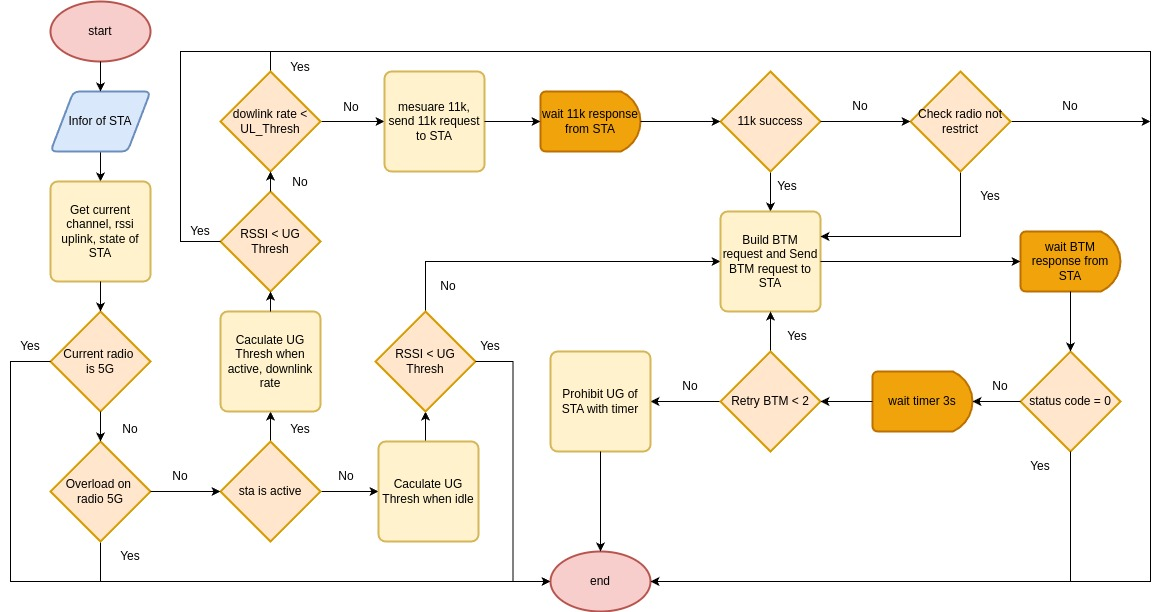
\includegraphics[width=1\textwidth]{mainmatter/images/UG_STEERING_VHT.jpg}
\caption{\label{fig:EasyMeshSystemModel}Lưu đồ thuật toán chuyển băng tần thấp lên cao trên AP}
\end{figure}

\begin{figure}
\centering
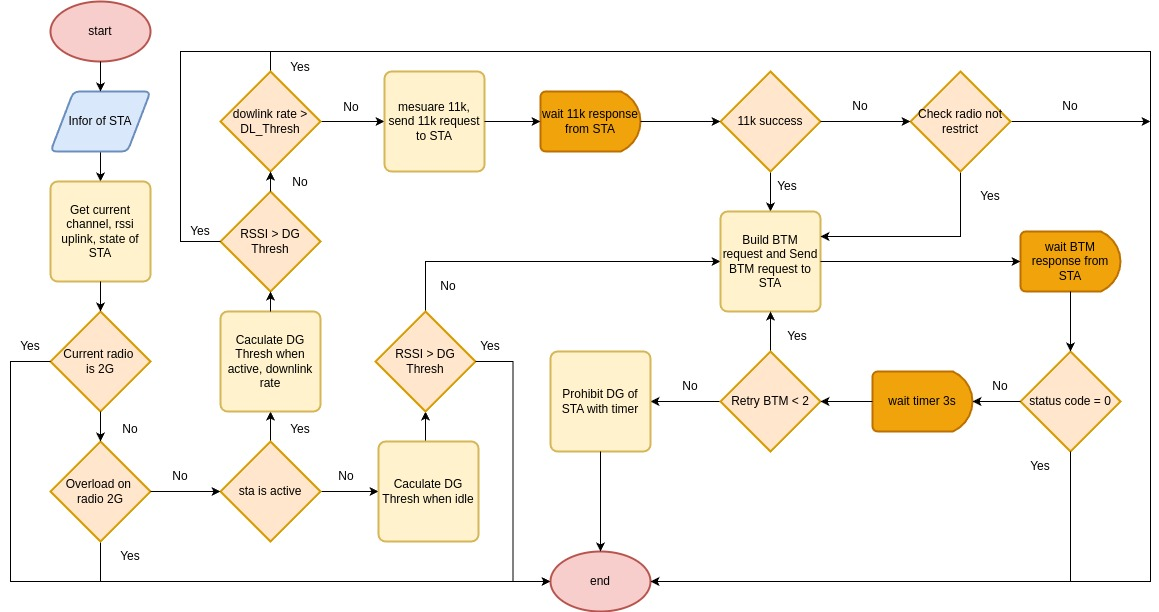
\includegraphics[width=1\textwidth]{mainmatter/images/DG_STEERING_VHT.jpg}
\caption{\label{fig:EasyMeshSystemModel}Lưu đồ thuật toán chuyển băng tần cao xuống thấp trên AP}
\end{figure}

\begin{figure}
\centering
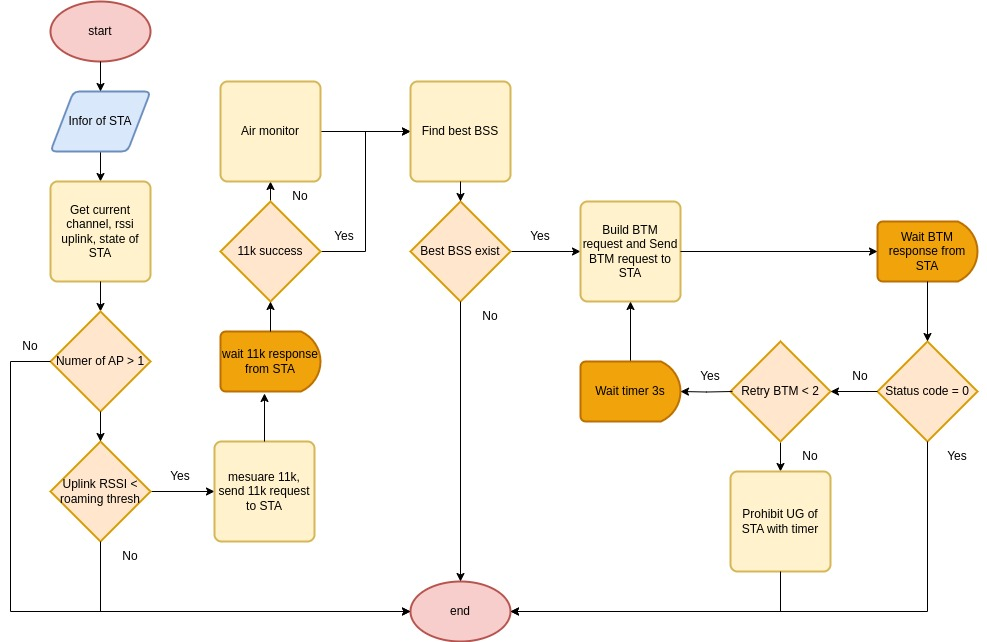
\includegraphics[width=1\textwidth]{mainmatter/images/Roaming_VHT.jpg}
\caption{\label{fig:EasyMeshSystemModel}Lưu đồ thuật toán chuyển vùng giữa AP}
\end{figure}
\end{center}

\section{Thuật toán chuyển vùng giữa các AP}
\begin{enumerate}
\item Thực hiện cập nhật thông tin kết nối giữa bộ phát sóng và thiết bị kết nối với nó định kỳ, thông tin này bao gồm cường độ tín hiệu, băng tần đang sử dụng để kết nối.
\item Đánh giá tình trạng kết nối của thiết bị kết nối không dây trong mạng để quyết định xem có tiến hành thực hiện chuyển vùng cho thiết bị đó hay không?. Việc xem xét thực hiện chuyển vùng cho thiết bị kết nối được quyết định theo công thức sau:
\item Nếu x < y thì thực hiện tiếp bước 3 để tìm vùng phủ mới cho thiết bị chuyển vùng đến và ngược lại thì thiết bị vẫn đang có kết nối đủ tốt đến vùng phủ hiện tại nên bỏ qua và thực hiện đánh giá với thiết bị khác. Nếu không cần thực hiện chuyển vùng thì quay lại bước 1. Trong trường hợp thiết bị cần chuyển vùng, bộ phát sóng mà thiết bị đang kết nối sẽ kích hoạt cơ chế gửi bản tin yêu cầu thông tin kết nối từ thiết bị tới các bộ phát sóng khác trong mạng. Thiết bị sẽ gửi bản tin phản hồi chứa thông tin kết nối từ thiết bị này đến các bộ phát sóng khác mà nó có thể quét được cho bộ phát sóng đang kết nối tới thiết bị. Từ đó có dữ liệu để thực hiện tìm kiếm vùng phủ sóng thích hợp cho thiết bị chuyển vùng tới.
\item Sau khi có thông tin về kết nối của thiết bị với các bộ phát sóng khác, thực hiện thuật toán tìm kiếm vùng phủ mới phù hợp cho thiết bị kết nối tới. Bộ phát sóng mà thiết bị đang kết nối sẽ chạy thuật toán tìm kiếm vùng phủ lân cận của nó để chuyển vùng cho thiết bị sang một trong số các vùng phủ lân cận phát bởi các bộ phát sóng trong mạng. Đầu tiên, các dữ liệu liên quan đến cường độ tín hiệu giữa các bộ phát sóng được đánh giá, nếu bộ phát sóng đang xem xét cho cường độ tín hiệu còn thấp hơn bộ phát sóng hiện tại thì sẽ thực hiện bỏ qua và xét tiếp đến các bộ phát sóng tiếp theo. Nếu bộ phát sóng đang xét cho cường độ tín hiệu tốt hơn, thực hiện tính giá trị  của các bộ phát sóng theo công thức đã được định nghĩa tại (5)(6) và tìm giá trị  lớn nhất trong các bộ phát sóng này. Sau khi tìm được bộ phát có giá trị  tốt nhất, thực hiện tìm vùng phủ sóng có khả năng chiếm dụng kênh lớn nhất trong các vùng phủ được phát bởi bộ phát sóng. Kết thúc quá trình tìm kiếm, ta thu được thông tin của vùng phủ mới phù hợp để chuyển vùng cho thiết bị kết nối tới.
\item Khi trạm phát tìm được vùng phủ sóng mới để thiết bị đang kết nối thực hiện chuyển vùng, nó sẽ gửi bản tin yêu cầu chuyển vùng (Request for Steering, RFS Request) sang bộ phát sóng chứa vùng phủ đích mà thiết bị sẽ kết nối tới. Mô hình luồng bản tin tại bước 4 và bước 5 được mô tả trong hình 2. Chi tiết nội dung bản tin này được mô tả trong bảng 5.
Khi bộ phát sóng nhận được bản tin RFS Request này, bộ phát sóng sẽ gửi lại bản tin phản hồi chuyển vùng (RFS Response) để trả lời việc có cho phép thiết bị có được chuyển vùng sang vùng phủ của nó hay không. Nếu được phép thì thiết bị kết nối sẽ được kích hoạt quá trình chuyển vùng và ngược lại thì yêu cầu chuyển vùng này bị bỏ qua. Chi tiết nội dung bản tin RFS Response được mô tả trong bảng 6:
\item Sau khi bộ phát nhận được bản tin RFS Response chấp thuận cho việc chuyển vùng của thiết bị, bộ phát sóng sẽ gửi bản tin quản lý chuyển dịch vùng phủ (BSS Transition Management, BTM) tới thiết bị để yêu cầu chuyển kết nối sang vùng phủ mới. Bản tin BTM Request cung cấp thông tin cho thiết bị khách về những bộ phát sóng mà có thể hỗ trợ nó có thể chuyển vùng tới được mô tả tại bảng 7. Khi thiết bị nhận được bản tin BTM này, thiết bị sẽ thực hiện chuyển vùng sang vùng phủ sóng mới mà nó được yêu cầu chuyển sang. Thiết bị sẽ gửi lại bản tin phản hồi quản lý chuyển vùng (BTM Response) để báo cáo quá trình chuyển vùng có thành công hay không. Nếu quá thời gian hạn định mà không nhận được bản tin BTM Response này, bộ phát sóng sẽ thực hiện gửi lại bản tin BTM. Chi tiết bản tin nôi dung bản tin BTM Response được mô tả trong bảng 8: Khi nhận được bản tin thông báo có thiết bị kết nối mới từ bộ phát sóng mà thiết bị chuyển vùng tới, bộ phát sóng kết nối với thiết bị lúc trước sẽ gửi bản tin yêu cầu kết thúc quá trình chuyển vùng (Teardown Steering Request, TSQ Request) tới bộ phát sóng mà thiết bị đã chuyển vùng tới. Chi tiết bản tin thông báo có thiết bị kết nối mới được mô tả ở bảng 9. Nếu quá thời gian hạn định không nhận được bản tin phản hồi (TSQ Response), bộ phát sóng sẽ gửi lại TSQ Request. Khi bộ phát sóng nhận được TSQ Response, quá trình chuyển vùng cho thiết bị sẽ kết thúc. Chi tiết bản tin TSQ Response được mô tả trong bảng 11:
\end{enumerate}

\section{Phân tích mã nguồn EasyMesh}